\documentclass{IEEEcsmag}

\usepackage[colorlinks,urlcolor=blue,linkcolor=blue,citecolor=blue]{hyperref}
\expandafter\def\expandafter\UrlBreaks\expandafter{\UrlBreaks\do\/\do\*\do\-\do\~\do\'\do\''\do\-}
\usepackage{upmath,color}

%%\usepackage{draftwatermark}
%%\SetWatermarkText{DRAFT}


\jvol{XX}
\jnum{XX}
\paper{8}
\jmonth{Month}
\jname{\textit{IEEE Annals of the History of Computing}}
\jtitle{\textit{IEEE Annals of the History of Computing}}
\pubyear{2025}

\newtheorem{theorem}{Theorem}
\newtheorem{lemma}{Lemma}


\setcounter{secnumdepth}{0}

\begin{document}

\sptitle{ARTICLE}

\title{The First Fifteen Years of Computing in Aotearoa New Zealand}

\author{Brian E. Carpenter}
\affil{University of Auckland, New Zealand}

\author{Sathiamoorthy Manoharan}
\affil{University of Auckland, New Zealand}

\author{Janet Toland}
\affil{Victoria University of Wellington, New Zealand}


\markboth{ARTICLE}{ARTICLE}

\begin{abstract}This article outlines the first fifteen years of modern computing in New Zealand ... 
\end{abstract}

\maketitle


\chapteri{M}odern computers arrived in Aotearoa New Zealand in 1960, little over a century after the first discernable information technology \cite{pioneers}. New Zealand was then a relatively isolated and small (2.5 million people) economy, so it is feasible to track the dissemination and socio-economic influence of computing for the following period; this study runs from 1960 to about 1975. Two events in the mid-1970s signaled the end of the economic and social era that began after World War II, and act as the end of our study: Britain joined the European Common Market in 1973, with major economic consequences, and New Zealand switched on a national Police Computer in 1976, with significant social impact.

In 1960, New Zealand had a rather centrally managed economy. Indeed, its currency did not float until as late as 1985. The details are complex \cite{Sullivan2013}, but the result was that during the period of our study the Treasury was constantly concerned about the foreign exchange impact of computer imports, and this necessitated a system of import licensing. This was a constant background for trends in computing, especially since the Treasury initially favored computing service bureaus to ensure maximum usage of what they considered a scarce resource. Of course, many companies much preferred to have their own systems.

Several themes are used to organize this article:

\begin{itemize}
\item growth in numbers of computers and vendors
\item growth in employees (and male dominance?) (and Pākehā/Māori?)
\item types of usage, including service bureaus
\item key areas where the technology was used
\item local contributions to the technology 
\item start of computing services and teaching in universities, technical colleges (and maybe schools?)
\item professionalization (NZCS)
\item commercial impact
\item social impact
\end{itemize}

\vspace*{-8pt}
\section{GROWTH IN NUMBERS AND EMPLOYMENT}

The following table shows the estimated number of electronic digital computers installed in New Zealand over the years in question.

\begin{center}
\begin{tabular}{ |c|c|c|c| } 
 \hline
 Year & Computers & Source & Notes\\ 
\hline
1960 & 2 & \cite{FirstCinNZ}&\\ 
1965 & 70 & \cite{Beardon} & \cite{HoneHeke} gives 45\\ 
1966 & 81 & \cite{Beardon}&\\
1968 & 120 & \cite{Beardon} & \cite{Yearbook75} gives 87\\
1969 & 140 & \cite{Beardon}&\\
1971 & 180 & \cite{Beardon}&\\
1972 & 200 & \cite{Yearbook75}&\\
1974 & 280 & \cite{Beardon}&\\
1976 & 400 & \cite{Beardon}&\\
 \hline
\end{tabular}
\end{center}

Although there are some discrepancies in the available data, the trend is one of rapid growth, from one computer for every 1.2 million people to one for every 8000. Similarly, the number of programmers in public services rose from a handful (maybe 4) in 1960 to 115 (84 men and
31 women) by 1974 \cite{Yearbook75}. Overall, 4000 data processing staff were then employed at  220 sites -- 39\% in Wellington, 31\% in Auckland, 9\% elsewhere in the North Island, and 21\% in the South Island \cite{Beardon}.

[discuss active companies (IBM, ICT/ICL and the rest), and popular models]

Throughout the period under study, most computers remained large and comparatively heavy, even as they moved from ``first generation'' (vacuum tubes) through ``second generation'' (discrete transistors) and ``third generation'' (integrated circuits) to the ``fourth generation'' (very large scale integration). As the technology got smaller, mainframe computers became more powerful rather than more compact. For example, the third computer installed in 1969 by Motor Specialties in Auckland, an ICL 1902A, needed to be lifted to the top floor by crane, like its predecessors , an ICT 1201 and an ICT 1301 (Figure~\ref{MS1902A}). 

\begin{figure}
\centerline{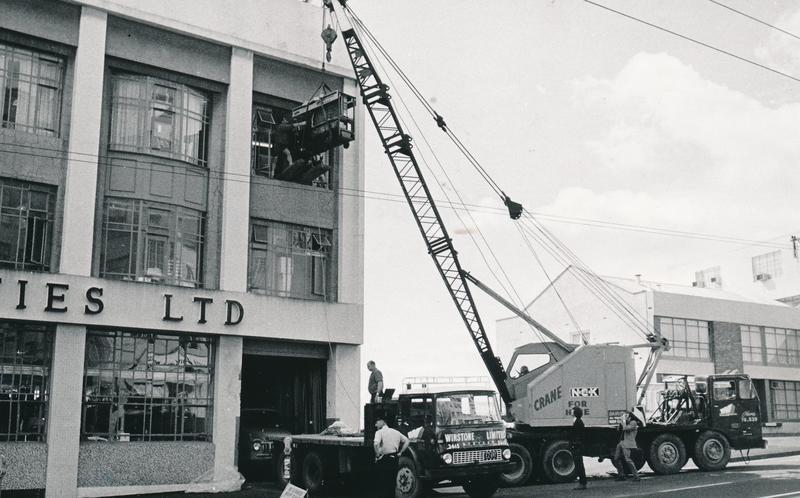
\includegraphics[width=18.5pc]{MotorSpec1902A-1969.jpg}}
\caption{\label{MS1902A}ICL 1902A Delivery in 1969. Courtesy Fletcher Archives, NZ.}\vspace*{-5pt}
\end{figure}

TBD
\vspace*{-8pt}
\section{CONCLUSION}

TBD

\vspace*{-8pt}
\section{ACKNOWLEDGMENTS}

TBD

%% style ieeetr doesn't display all details or alphabetise
%% style IEEEtran doesn't alphabetise
%% style plain doesn't meet IEEE requirements
\bibliographystyle{IEEEtranS}
\bibliography{growth}

\begin{IEEEbiography}{Brian E. Carpenter} is an Honorary Professor in the School of Computer Science, University of Auckland, New Zealand. He is interested in Internet protocol design and in computing history. He received a Ph.D. from the University of Manchester, U.K. and is a past Chair of the Internet Engineering Task Force. Contact: brian@cs.auckland.ac.nz\vspace*{8pt}
\end{IEEEbiography}

\begin{IEEEbiography}{Sathiamoorthy Manoharan} is a Senior Lecturer in the School of Computer Science, University of Auckland, New Zealand.
He is a senior member of IEEE. He is interested in computer systems, particularly with respect to performance and security. Contact: mano.manoharan@auckland.ac.nz.\vspace*{8pt}
\end{IEEEbiography}

\begin{IEEEbiography}{Janet Toland} is currently an Associate Professor in the
School of Information Management, Te Herenga Waka, Victoria
University of Wellington, Wellington, New Zealand. Her
research work is in the history of information systems. She
has a particular interest in social and ethical issues. She is
currently the Historian for the Association of Information
Systems. Contact her at Janet.Toland@vuw.ac.nz.\vspace*{8pt}
\end{IEEEbiography}



\end{document}

